\documentclass[11pt]{article}

\usepackage{UCLAhandout_aditya}
\usepackage{course}
%%%%% NEW MATH DEFINITIONS %%%%%

\usepackage{amsmath,amsfonts,bm}

% Mark sections of captions for referring to divisions of figures
\newcommand{\figleft}{{\em (Left)}}
\newcommand{\figcenter}{{\em (Center)}}
\newcommand{\figright}{{\em (Right)}}
\newcommand{\figtop}{{\em (Top)}}
\newcommand{\figbottom}{{\em (Bottom)}}
\newcommand{\captiona}{{\em (a)}}
\newcommand{\captionb}{{\em (b)}}
\newcommand{\captionc}{{\em (c)}}
\newcommand{\captiond}{{\em (d)}}

% Highlight a newly defined term
\newcommand{\newterm}[1]{{\bf #1}}


% Figure reference, lower-case.
\def\figref#1{figure~\ref{#1}}
% Figure reference, capital. For start of sentence
\def\Figref#1{Figure~\ref{#1}}
\def\twofigref#1#2{figures \ref{#1} and \ref{#2}}
\def\quadfigref#1#2#3#4{figures \ref{#1}, \ref{#2}, \ref{#3} and \ref{#4}}
% Section reference, lower-case.
\def\secref#1{section~\ref{#1}}
% Section reference, capital.
\def\Secref#1{Section~\ref{#1}}
% Reference to two sections.
\def\twosecrefs#1#2{sections \ref{#1} and \ref{#2}}
% Reference to three sections.
\def\secrefs#1#2#3{sections \ref{#1}, \ref{#2} and \ref{#3}}
% Reference to an equation, lower-case.
% \def\eqref#1{equation~\ref{#1}}
% Reference to an equation, upper case
\def\Eqref#1{Equation~\ref{#1}}
% A raw reference to an equation---avoid using if possible
\def\plaineqref#1{\ref{#1}}
% Reference to a chapter, lower-case.
\def\chapref#1{chapter~\ref{#1}}
% Reference to an equation, upper case.
\def\Chapref#1{Chapter~\ref{#1}}
% Reference to a range of chapters
\def\rangechapref#1#2{chapters\ref{#1}--\ref{#2}}
% Reference to an algorithm, lower-case.
\def\algref#1{algorithm~\ref{#1}}
% Reference to an algorithm, upper case.
\def\Algref#1{Algorithm~\ref{#1}}
\def\twoalgref#1#2{algorithms \ref{#1} and \ref{#2}}
\def\Twoalgref#1#2{Algorithms \ref{#1} and \ref{#2}}
% Reference to a part, lower case
\def\partref#1{part~\ref{#1}}
% Reference to a part, upper case
\def\Partref#1{Part~\ref{#1}}
\def\twopartref#1#2{parts \ref{#1} and \ref{#2}}

\def\ceil#1{\lceil #1 \rceil}
\def\floor#1{\lfloor #1 \rfloor}
\def\1{\bm{1}}
\newcommand{\train}{D_{\mathrm{train}}}
\newcommand{\valid}{D_{\mathrm{valid}}}
\newcommand{\test}{D_{\mathrm{test}}}

% \newcommand{\train}{\mathcal{D}}
% \newcommand{\valid}{\mathcal{D_{\mathrm{valid}}}}
% \newcommand{\test}{\mathcal{D_{\mathrm{test}}}}

\def\eps{{\epsilon}}
\def\fid{{\textnormal{FID}}}


\def\calX{{\mathcal{X}}}
\def\calY{{\mathcal{Y}}}
\def\calZ{{\mathcal{Z}}}
\def\gxy{G_{\mathcal{X} \rightarrow  \mathcal{Y}}}
\def\gyx{G_{\mathcal{Y} \rightarrow  \mathcal{X}}}
\def\gzx{G_{\mathcal{Z} \rightarrow  \mathcal{X}}}
\def\gxz{G_{\mathcal{X} \rightarrow  \mathcal{Z}}}
\def\gzy{G_{\mathcal{Z} \rightarrow  \mathcal{Y}}}
\def\gyz{G_{\mathcal{Y} \rightarrow  \mathcal{Z}}}

% Random variables
% \def\reta{{\textnormal{$\eta$}}}
% \def\ra{{\textnormal{a}}}
% \def\rb{{\textnormal{b}}}
% \def\rc{{\textnormal{c}}}
% \def\rd{{\textnormal{d}}}
% \def\re{{\textnormal{e}}}
% \def\rf{{\textnormal{f}}}
% \def\rg{{\textnormal{g}}}
% \def\rh{{\textnormal{h}}}
% \def\ri{{\textnormal{i}}}
% \def\rj{{\textnormal{j}}}
% \def\rk{{\textnormal{k}}}
% \def\rl{{\textnormal{l}}}
% % rm is already a command, just don't name any random variables m
% \def\rn{{\textnormal{n}}}
% \def\ro{{\textnormal{o}}}
% \def\rp{{\textnormal{p}}}
% \def\rq{{\textnormal{q}}}
% \def\rr{{\textnormal{r}}}
% \def\rs{{\textnormal{s}}}
% \def\rt{{\textnormal{t}}}
% \def\ru{{\textnormal{u}}}
% \def\rv{{\textnormal{v}}}
% \def\rw{{\textnormal{w}}}
% \def\rx{{\textnormal{x}}}
% \def\ry{{\textnormal{y}}}
% \def\rz{{\textnormal{z}}}

\def\rx{{\textnormal{X}}}
\def\ry{{\textnormal{Y}}}
\def\rz{{\textnormal{Z}}}

% Random vectors
% \def\rvepsilon{{\mathbf{\epsilon}}}
% \def\rvtheta{{\mathbf{\theta}}}
% \def\rva{{\mathbf{a}}}
% \def\rvb{{\mathbf{b}}}
% \def\rvc{{\mathbf{c}}}
% \def\rvd{{\mathbf{d}}}
% \def\rve{{\mathbf{e}}}
% \def\rvf{{\mathbf{f}}}
% \def\rvg{{\mathbf{g}}}
% \def\rvh{{\mathbf{h}}}
% \def\rvu{{\mathbf{i}}}
% \def\rvj{{\mathbf{j}}}
% \def\rvk{{\mathbf{k}}}
% \def\rvl{{\mathbf{l}}}
% \def\rvm{{\mathbf{m}}}
% \def\rvn{{\mathbf{n}}}
% \def\rvo{{\mathbf{o}}}
% \def\rvp{{\mathbf{p}}}
% \def\rvq{{\mathbf{q}}}
% \def\rvr{{\mathbf{r}}}
% \def\rvs{{\mathbf{s}}}
% \def\rvt{{\mathbf{t}}}
% \def\rvu{{\mathbf{u}}}
% \def\rvv{{\mathbf{v}}}
% \def\rvw{{\mathbf{w}}}
% \def\rvx{{\mathbf{x}}}
% \def\rvy{{\mathbf{y}}}
% \def\rvz{{\mathbf{z}}}

\def\rvx{{\mathbf{X}}}
\def\rvy{{\mathbf{Y}}}
\def\rvz{{\mathbf{Z}}}

% Elements of random vectors
\def\erva{{\textnormal{a}}}
\def\ervb{{\textnormal{b}}}
\def\ervc{{\textnormal{c}}}
\def\ervd{{\textnormal{d}}}
\def\erve{{\textnormal{e}}}
\def\ervf{{\textnormal{f}}}
\def\ervg{{\textnormal{g}}}
\def\ervh{{\textnormal{h}}}
\def\ervi{{\textnormal{i}}}
\def\ervj{{\textnormal{j}}}
\def\ervk{{\textnormal{k}}}
\def\ervl{{\textnormal{l}}}
\def\ervm{{\textnormal{m}}}
\def\ervn{{\textnormal{n}}}
\def\ervo{{\textnormal{o}}}
\def\ervp{{\textnormal{p}}}
\def\ervq{{\textnormal{q}}}
\def\ervr{{\textnormal{r}}}
\def\ervs{{\textnormal{s}}}
\def\ervt{{\textnormal{t}}}
\def\ervu{{\textnormal{u}}}
\def\ervv{{\textnormal{v}}}
\def\ervw{{\textnormal{w}}}
\def\ervx{{\textnormal{x}}}
\def\ervy{{\textnormal{y}}}
\def\ervz{{\textnormal{z}}}

% Random matrices
\def\rmA{{\mathbf{A}}}
\def\rmB{{\mathbf{B}}}
\def\rmC{{\mathbf{C}}}
\def\rmD{{\mathbf{D}}}
\def\rmE{{\mathbf{E}}}
\def\rmF{{\mathbf{F}}}
\def\rmG{{\mathbf{G}}}
\def\rmH{{\mathbf{H}}}
\def\rmI{{\mathbf{I}}}
\def\rmJ{{\mathbf{J}}}
\def\rmK{{\mathbf{K}}}
\def\rmL{{\mathbf{L}}}
\def\rmM{{\mathbf{M}}}
\def\rmN{{\mathbf{N}}}
\def\rmO{{\mathbf{O}}}
\def\rmP{{\mathbf{P}}}
\def\rmQ{{\mathbf{Q}}}
\def\rmR{{\mathbf{R}}}
\def\rmS{{\mathbf{S}}}
\def\rmT{{\mathbf{T}}}
\def\rmU{{\mathbf{U}}}
\def\rmV{{\mathbf{V}}}
\def\rmW{{\mathbf{W}}}
\def\rmX{{\mathbf{X}}}
\def\rmY{{\mathbf{Y}}}
\def\rmZ{{\mathbf{Z}}}

% Elements of random matrices
\def\ermA{{\textnormal{A}}}
\def\ermB{{\textnormal{B}}}
\def\ermC{{\textnormal{C}}}
\def\ermD{{\textnormal{D}}}
\def\ermE{{\textnormal{E}}}
\def\ermF{{\textnormal{F}}}
\def\ermG{{\textnormal{G}}}
\def\ermH{{\textnormal{H}}}
\def\ermI{{\textnormal{I}}}
\def\ermJ{{\textnormal{J}}}
\def\ermK{{\textnormal{K}}}
\def\ermL{{\textnormal{L}}}
\def\ermM{{\textnormal{M}}}
\def\ermN{{\textnormal{N}}}
\def\ermO{{\textnormal{O}}}
\def\ermP{{\textnormal{P}}}
\def\ermQ{{\textnormal{Q}}}
\def\ermR{{\textnormal{R}}}
\def\ermS{{\textnormal{S}}}
\def\ermT{{\textnormal{T}}}
\def\ermU{{\textnormal{U}}}
\def\ermV{{\textnormal{V}}}
\def\ermW{{\textnormal{W}}}
\def\ermX{{\textnormal{X}}}
\def\ermY{{\textnormal{Y}}}
\def\ermZ{{\textnormal{Z}}}

% Vectors
% \def\vzero{{\bm{0}}}
% \def\vone{{\bm{1}}}
% \def\vmu{{\bm{\mu}}}
% \def\vtheta{{\bm{\theta}}}
% \def\va{{\bm{a}}}
% \def\vb{{\bm{b}}}
% \def\vc{{\bm{c}}}
% \def\vd{{\bm{d}}}
% \def\ve{{\bm{e}}}
% \def\vf{{\bm{f}}}
% \def\vg{{\bm{g}}}
% \def\vh{{\bm{h}}}
% \def\vi{{\bm{i}}}
% \def\vj{{\bm{j}}}
% \def\vk{{\bm{k}}}
% \def\vl{{\bm{l}}}
% \def\vm{{\bm{m}}}
% \def\vn{{\bm{n}}}
% \def\vo{{\bm{o}}}
% \def\vp{{\bm{p}}}
% \def\vq{{\bm{q}}}
% \def\vr{{\bm{r}}}
% \def\vs{{\bm{s}}}
% \def\vt{{\bm{t}}}
% \def\vu{{\bm{u}}}
% \def\vv{{\bm{v}}}
% \def\vw{{\bm{w}}}
% \def\vx{{\bm{x}}}
% \def\vy{{\bm{y}}}
% \def\vz{{\bm{z}}}
\def\va{{\mathbf{a}}}
\def\vs{{\mathbf{s}}}
\def\vx{{\mathbf{x}}}
\def\vy{{\mathbf{y}}}
\def\vz{{\mathbf{z}}}

% Elements of vectors
\def\evalpha{{\alpha}}
\def\evbeta{{\beta}}
\def\evepsilon{{\epsilon}}
\def\evlambda{{\lambda}}
\def\evomega{{\omega}}
\def\evmu{{\mu}}
\def\evpsi{{\psi}}
\def\evsigma{{\sigma}}
\def\evtheta{{\theta}}
\def\eva{{a}}
\def\evb{{b}}
\def\evc{{c}}
\def\evd{{d}}
\def\eve{{e}}
\def\evf{{f}}
\def\evg{{g}}
\def\evh{{h}}
\def\evi{{i}}
\def\evj{{j}}
\def\evk{{k}}
\def\evl{{l}}
\def\evm{{m}}
\def\evn{{n}}
\def\evo{{o}}
\def\evp{{p}}
\def\evq{{q}}
\def\evr{{r}}
\def\evs{{s}}
\def\evt{{t}}
\def\evu{{u}}
\def\evv{{v}}
\def\evw{{w}}
\def\evx{{x}}
\def\evy{{y}}
\def\evz{{z}}

% Matrix
\def\mA{{\bm{A}}}
\def\mB{{\bm{B}}}
\def\mC{{\bm{C}}}
\def\mD{{\bm{D}}}
\def\mE{{\bm{E}}}
\def\mF{{\bm{F}}}
\def\mG{{\bm{G}}}
\def\mH{{\bm{H}}}
\def\mI{{\bm{I}}}
\def\mJ{{\bm{J}}}
\def\mK{{\bm{K}}}
\def\mL{{\bm{L}}}
\def\mM{{\bm{M}}}
\def\mN{{\bm{N}}}
\def\mO{{\bm{O}}}
\def\mP{{\bm{P}}}
\def\mQ{{\bm{Q}}}
\def\mR{{\bm{R}}}
\def\mS{{\bm{S}}}
\def\mT{{\bm{T}}}
\def\mU{{\bm{U}}}
\def\mV{{\bm{V}}}
\def\mW{{\bm{W}}}
\def\mX{{\bm{X}}}
\def\mY{{\bm{Y}}}
\def\mZ{{\bm{Z}}}
\def\mBeta{{\bm{\beta}}}
\def\mPhi{{\bm{\Phi}}}
\def\mLambda{{\bm{\Lambda}}}
\def\mSigma{{\bm{\Sigma}}}

% Tensor
\DeclareMathAlphabet{\mathsfit}{\encodingdefault}{\sfdefault}{m}{sl}
\SetMathAlphabet{\mathsfit}{bold}{\encodingdefault}{\sfdefault}{bx}{n}
\newcommand{\tens}[1]{\bm{\mathsfit{#1}}}
\def\tA{{\tens{A}}}
\def\tB{{\tens{B}}}
\def\tC{{\tens{C}}}
\def\tD{{\tens{D}}}
\def\tE{{\tens{E}}}
\def\tF{{\tens{F}}}
\def\tG{{\tens{G}}}
\def\tH{{\tens{H}}}
\def\tI{{\tens{I}}}
\def\tJ{{\tens{J}}}
\def\tK{{\tens{K}}}
\def\tL{{\tens{L}}}
\def\tM{{\tens{M}}}
\def\tN{{\tens{N}}}
\def\tO{{\tens{O}}}
\def\tP{{\tens{P}}}
\def\tQ{{\tens{Q}}}
\def\tR{{\tens{R}}}
\def\tS{{\tens{S}}}
\def\tT{{\tens{T}}}
\def\tU{{\tens{U}}}
\def\tV{{\tens{V}}}
\def\tW{{\tens{W}}}
\def\tX{{\tens{X}}}
\def\tY{{\tens{Y}}}
\def\tZ{{\tens{Z}}}


% Graph
\def\gA{{\mathcal{A}}}
\def\gB{{\mathcal{B}}}
\def\gC{{\mathcal{C}}}
\def\gD{{\mathcal{D}}}
\def\gE{{\mathcal{E}}}
\def\gF{{\mathcal{F}}}
\def\gG{{\mathcal{G}}}
\def\gH{{\mathcal{H}}}
\def\gI{{\mathcal{I}}}
\def\gJ{{\mathcal{J}}}
\def\gK{{\mathcal{K}}}
\def\gL{{\mathcal{L}}}
\def\gM{{\mathcal{M}}}
\def\gN{{\mathcal{N}}}
\def\gO{{\mathcal{O}}}
\def\gP{{\mathcal{P}}}
\def\gQ{{\mathcal{Q}}}
\def\gR{{\mathcal{R}}}
\def\gS{{\mathcal{S}}}
\def\gT{{\mathcal{T}}}
\def\gU{{\mathcal{U}}}
\def\gV{{\mathcal{V}}}
\def\gW{{\mathcal{W}}}
\def\gX{{\mathcal{X}}}
\def\gY{{\mathcal{Y}}}
\def\gZ{{\mathcal{Z}}}

% Sets
\def\sA{{\mathbb{A}}}
\def\sB{{\mathbb{B}}}
\def\sC{{\mathbb{C}}}
\def\sD{{\mathbb{D}}}
% Don't use a set called E, because this would be the same as our symbol
% for expectation.
\def\sF{{\mathbb{F}}}
\def\sG{{\mathbb{G}}}
\def\sH{{\mathbb{H}}}
\def\sI{{\mathbb{I}}}
\def\sJ{{\mathbb{J}}}
\def\sK{{\mathbb{K}}}
\def\sL{{\mathbb{L}}}
\def\sM{{\mathbb{M}}}
\def\sN{{\mathbb{N}}}
\def\sO{{\mathbb{O}}}
\def\sP{{\mathbb{P}}}
\def\sQ{{\mathbb{Q}}}
\def\sR{{\mathbb{R}}}
\def\sS{{\mathbb{S}}}
\def\sT{{\mathbb{T}}}
\def\sU{{\mathbb{U}}}
\def\sV{{\mathbb{V}}}
\def\sW{{\mathbb{W}}}
\def\sX{{\mathbb{X}}}
\def\sY{{\mathbb{Y}}}
\def\sZ{{\mathbb{Z}}}

% Entries of a matrix
\def\emLambda{{\Lambda}}
\def\emA{{A}}
\def\emB{{B}}
\def\emC{{C}}
\def\emD{{D}}
\def\emE{{E}}
\def\emF{{F}}
\def\emG{{G}}
\def\emH{{H}}
\def\emI{{I}}
\def\emJ{{J}}
\def\emK{{K}}
\def\emL{{L}}
\def\emM{{M}}
\def\emN{{N}}
\def\emO{{O}}
\def\emP{{P}}
\def\emQ{{Q}}
\def\emR{{R}}
\def\emS{{S}}
\def\emT{{T}}
\def\emU{{U}}
\def\emV{{V}}
\def\emW{{W}}
\def\emX{{X}}
\def\emY{{Y}}
\def\emZ{{Z}}
\def\emSigma{{\Sigma}}

% entries of a tensor
% Same font as tensor, without \bm wrapper
\newcommand{\etens}[1]{\mathsfit{#1}}
\def\etLambda{{\etens{\Lambda}}}
\def\etA{{\etens{A}}}
\def\etB{{\etens{B}}}
\def\etC{{\etens{C}}}
\def\etD{{\etens{D}}}
\def\etE{{\etens{E}}}
\def\etF{{\etens{F}}}
\def\etG{{\etens{G}}}
\def\etH{{\etens{H}}}
\def\etI{{\etens{I}}}
\def\etJ{{\etens{J}}}
\def\etK{{\etens{K}}}
\def\etL{{\etens{L}}}
\def\etM{{\etens{M}}}
\def\etN{{\etens{N}}}
\def\etO{{\etens{O}}}
\def\etP{{\etens{P}}}
\def\etQ{{\etens{Q}}}
\def\etR{{\etens{R}}}
\def\etS{{\etens{S}}}
\def\etT{{\etens{T}}}
\def\etU{{\etens{U}}}
\def\etV{{\etens{V}}}
\def\etW{{\etens{W}}}
\def\etX{{\etens{X}}}
\def\etY{{\etens{Y}}}
\def\etZ{{\etens{Z}}}

% The true underlying data generating distribution
\newcommand{\pdata}{p_{\rm{data}}}
% The empirical distribution defined by the training set
\newcommand{\ptrain}{\hat{p}_{\rm{data}}}
\newcommand{\Ptrain}{\hat{P}_{\rm{data}}}
% The model distribution
\newcommand{\ptheta}{p_{\theta}}
\newcommand{\Ptheta}{P_{\theta}}
\newcommand{\ptildemodel}{\tilde{p}_{\theta}}
% \newcommand{\pmodel}{p_{\rm{model}}}
% \newcommand{\Pmodel}{P_{\rm{model}}}
% \newcommand{\ptildemodel}{\tilde{p}_{\rm{model}}}
% Stochastic autoencoder distributions
\newcommand{\pencode}{p_{\rm{encoder}}}
\newcommand{\pdecode}{p_{\rm{decoder}}}
\newcommand{\precons}{p_{\rm{reconstruct}}}

\newcommand{\laplace}{\mathrm{Laplace}} % Laplace distribution

% \newcommand{\E}{\mathbb{E}}
\newcommand{\Ls}{\mathcal{L}}
% \newcommand{\R}{\mathbb{R}}
\newcommand{\emp}{\tilde{p}}
\newcommand{\lr}{\alpha}
\newcommand{\reg}{\lambda}
\newcommand{\rect}{\mathrm{rectifier}}
\newcommand{\softmax}{\mathrm{softmax}}
\newcommand{\sigmoid}{\sigma}
\newcommand{\softplus}{\zeta}
\newcommand{\KL}{D_{\mathrm{KL}}}
\newcommand{\Var}{\mathrm{Var}}
\newcommand{\standarderror}{\mathrm{SE}}
\newcommand{\Cov}{\mathrm{Cov}}
% Wolfram Mathworld says $L^2$ is for function spaces and $\ell^2$ is for vectors
% But then they seem to use $L^2$ for vectors throughout the site, and so does
% wikipedia.
\newcommand{\normlzero}{L^0}
\newcommand{\normlone}{L^1}
\newcommand{\normltwo}{L^2}
\newcommand{\normlp}{L^p}
\newcommand{\normmax}{L^\infty}

\newcommand{\parents}{Pa} % See usage in notation.tex. Chosen to match Daphne's book.

% \DeclareMathOperator*{\argmax}{arg\,max}
% \DeclareMathOperator*{\argmin}{arg\,min}

\DeclareMathOperator{\sign}{sign}
\DeclareMathOperator{\Tr}{Tr}
\let\ab\allowbreak



\usepackage{color,amssymb,stmaryrd,amsmath,amsfonts,rotating,mathrsfs,psfrag}


\begin{document}

\handout{25th April 2023}{\Large Homework \#2 \\\small Due: 10th May 2023, Wednesday, before 11:59 pm}

\vspace{-0.5in}

\exercise[Decision Trees] \totalpoints{15}

You are checking the weather and would like to know whether a day is comfortable or not (IsComfortable). This is determined by factors such as whether a day is sunny (IsSunny), whether a day is hot (IsHot), etc. You have the following data to consider.

\begin{table}[H]
\centering
\begin{tabular}{|c|cccc|c|}
\hline
Example & IsSunny & IsHot & IsHumid & IsWindy & IsComfortable \\ \hline \hline
A & 0 & 0 & 0 & 0 & 0 \\
B & 0 & 0 & 1 & 0 & 0 \\
C & 1 & 1 & 0 & 1 & 0 \\
D & 1 & 0 & 0 & 1 & 1 \\
E & 0 & 1 & 1 & 0 & 1 \\
F & 0 & 0 & 1 & 1 & 1 \\
G & 0 & 0 & 0 & 1 & 1 \\
H & 1 & 0 & 1 & 1 & 1 \\ \hline
U & 1 & 1 & 1 & 1 & ? \\
V & 0 & 1 & 0 & 1 & ? \\
W & 1 & 1 & 0 & 0 & ? \\ \hline
\end{tabular}
\end{table}

You know whether or not a day A through H is comfortable, but you do not know about U through W. For questions (a) - (d), consider only days A through H. For all calculations in this problem, use base 2 for the logarithms.

\begin{enumerate}
\item \points{1} What is the entropy of IsComfortable? \vspace{2cm}

\item \points{1} Which attribute should you choose as the root of a decision tree? \vspace{3cm}

\item \points{5}  What is the information gain of the attribute you chose in the previous question? \vspace{6cm}
 
\item \points{5}  Using ID3 algorithm, build a decision tree to classify days as comfortable or not. \vspace{8cm}

\item \points{3} Classify days U, V and W using this decision tree as comfortable or not. 

\end{enumerate}

\newpage
\exercise[Entropy and Information]
\totalpoints{5}

The entropy of a Bernoulli (Boolean 0/1) random variable $X$ with $p(X = 1) = q$ is given by
\begin{equation*}
B(q) = - q \log q - (1 - q) \log(1 - q).
\end{equation*}
Suppose that a set $S$ contains $p$ positive examples and $n$ negative examples. The entropy of $S$ is defined as $H(S) = B\left(\frac{p}{p+n}\right)$.

Based on an attribute $X_j$, we split the set $S$ into $k$ disjoint subsets $S_k$, with $p_k$ positive and $n_k$ negative examples in each. If the ratio $\tfrac{p_k}{p_k + n_k}$ is the same for all $k$, show that the information gain of this attribute is 0. 

\newpage
\exercise[$k$-Nearest Neighbors]
\totalpoints{25}

In the following questions, you will consider a $k$-nearest neighbor classifier using Euclidean
distance metric on a binary classification task. 
We assign the class of the test point to be the
class of the majority of the $k$ nearest neighbors. Below is the figure for dataset. Note that the annotated data points (from 1 to 5) belong to the test set, and the rest belong to the training set.
\begin{figure}[h]
    \centering
    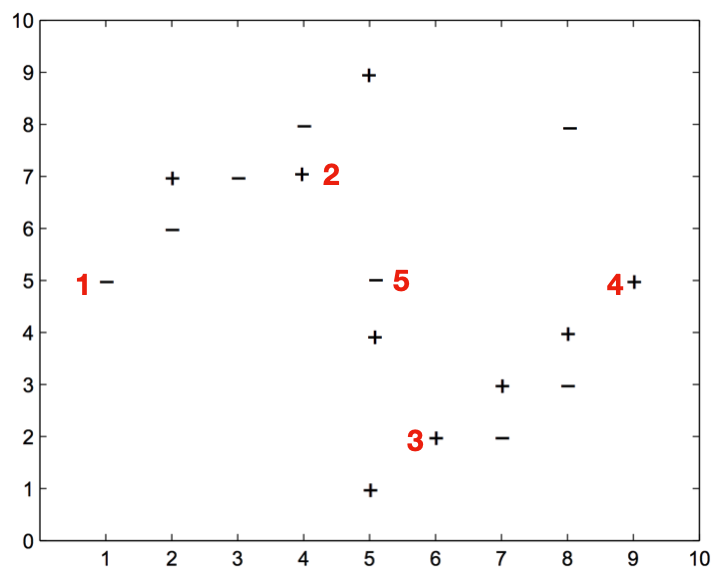
\includegraphics[scale=0.4]{figs/hw2_p32.png}
    \caption{Dataset for $k$NN binary classification task.}
    \label{fig:knn}
\end{figure}

\begin{enumerate}
\item \points{5} What value of $k$ minimizes the training set error? What is the resulting training error? Assume that for the purpose of computing nearest neighbors for the training set, a point can be its own neighbor. \vspace{2cm}


\item \points{10} In Figure \ref{fig:knn}, the points labelled as  ${\color{red}1, 2, 3, 4, 5}$ are test points, whereas all other points are training points.  Using the $k$ you obtained from question (a), what is the test error for the data points marked as ${\color{red}1, 2, 3, 4, 5}$ ? Clearly mention which points are misclassified. Note that a test point cannot be its own nearest neighbor as neighbors must belong to the training set. \newpage

\item[]

\item[] In the above parts, we had considered \textit{k}-nearest neighbor classifier using Euclidean distance metric. For the next part, we will choose \textit{cosine similarity} as a distance metric. We define cosine similarity between two vectors $\vect{u}, \vect{v}$ as:
$$sim(\vect{u}, \vect{v})  = \frac{ \langle \vect{u} , \vect{v} \rangle}{||\vect{u}||_{2}||\vect{v}||_{2}}$$
where $<\cdot,\cdot>$ is the inner product operator between two vectors, and $||.||_{2}$ is the $L_{2}$ norm operator. 

Note that for cosine similarity, we consider the nearest neighbors to be the points in the training set with the greatest cosine similarity (i.e. most similar points) to the test point.

[\emph{Hint}: Quoting from \href{https://en.wikipedia.org/wiki/Cosine_similarity}{Wikipedia}: ``Cosine similarity is the cosine of the angle between the vectors; that is, it is the dot product of the vectors divided by the product of their lengths. It follows that the cosine similarity does not depend on the magnitudes of the vectors, but only on their angle.'']

\item \points{10} Using the $k$ you choose from question (a), what is the test error for the data points marked as ${\color{red}1, 2, 3, 4, 5}$ in Figure \ref{fig:knn}? Clearly mention which points are misclassified. (Assume that a point is not its own neighbor). 

\end{enumerate}

\newpage
\exercise[Kernel Properties]
\totalpoints{15}

\begin{enumerate}
\item \points{5} Which of the following holds for any valid kernel function $k(\cdot,\cdot)$ and for all $\vect{u},\vect{v}$?
\begin{enumerate}
    \item $k(\vect{u},\vect{u})\ge 0$
    \item $k(\vect{u},\vect{v})\ge 0$
    \item $k(\vect{u}, \vect{u}) + k(\vect{v}, \vect{v})\ge 2k(\vect{u}, \vect{v})$
    \item $k(\vect{u}, \vect{u}) + k(\vect{v}, \vect{v})\ge -2k(\vect{u}, \vect{v})$
\end{enumerate} \vspace{2cm}


\item \points{10}
Kernel functions can be characterized by an implicit mapping $\phi(\vct x)$ that transforms a feature vector $\vct x\in \mathbb{R}^d$ to a higher dimensional space $Q$ by giving the form of inner product in $Q$: $K(\vct x^{(i)},\vct x^{(j)})=\phi(\vct x^{(i)})^T\phi(\vct x^{(j)})$.\\
Assume we use the radial basis kernel function $K(\vct x^{(i)},\vct x^{(j)})=\exp\left(-\frac{1}{2}||\vct x^{(i)}-\vct x^{(j)}||^2\right)$. So we assume that there is some implicit unknown function $\phi(\vct x)$ such that $$\phi(\vct x^{(i)})^T\phi(\vct x^{(j)})=K(\vct x^{(i)},\vct x^{(j)})=\exp\left(-\frac{1}{2}||\vct x^{(i)}-\vct x^{(j)}||^2\right)$$

Prove that for any two inputs $\vct x^{(i)}$ and $\vct x^{(j)}$, the squared euclidean distance $d(\vct x^{(i)},\vct x^{(j)})$, between them in the higher dimensional feature space $Q$ is less than 2, i.e. prove (\ref{a}) and (\ref{b}) in the following:
    \begin{align}
    d(\vct x^{(i)},\vct x^{(j)})& =||\phi(\vct x^{(i)})-\phi(\vct x^{(j)})||_2^2 \nonumber\\
    & = K(\vct x^{(i)},\vct x^{(i)})+K(\vct x^{(j)},\vct x^{(j)})-2K(\vct x^{(i)},\vct x^{(j)}) \label{a}\\
    & <2 \label{b}
    \end{align}
\end{enumerate}
\newpage

\exercise[Programming Exercise: Applying Classification Models]

\totalpoints{40}

In this problem, we ask you to compare the classification models we have studied till now i.e., Decision trees, K-nearest neighbors, and Logistic regression. 
\section*{Introduction\footnote{This assignment is adapted from the UCI Machine learning repository, available at \url{https://archive.ics.uci.edu/ml/datasets/adult}.}}

This data was extracted from the 1994 Census bureau database by Ronny Kohavi and Barry Becker. For computational reasons, we have already extracted a relatively clean subset of the data for this homework. The prediction task is to determine whether a person makes over \$50K a year.

In this problem, we ask you to complete the analysis of what sorts of people were likely to earn more than \$50K a year. In particular, we ask you to apply the tools of machine learning to predict which individuals are more likely to have high income. 



\section*{Starter Files}
\vspace{-\baselineskip}
\rule{\textwidth}{1pt}
code and data
\begin{itemize}[nolistsep]
    \item \verb|Sp23-CS146-HW2.ipynb|. Instruction is here \footnote{ To run the notebook on Google Colab, check the first 3 cells in \verb|Sp23-CS146-HW2.ipynb|; otherwise, delete the first 3 cells.}.
    \item \verb|nutil.py|
    \item \verb|adult_subsample.csv|
\end{itemize}
documentation
\begin{itemize}[nolistsep]
\item Decision Tree Classifier: \\{\footnotesize \url{http://scikit-learn.org/stable/modules/generated/sklearn.tree.DecisionTreeClassifier.html}}
\item K-Nearest Neighbor Classifier: \\{\footnotesize \url{http://scikit-learn.org/stable/modules/generated/sklearn.neighbors.KNeighborsClassifier.html}} 
\item Logistic Regression: \\{\footnotesize \url{https://scikit-learn.org/stable/modules/generated/sklearn.linear_model.LogisticRegression.html}}
\item Cross-Validation: \\{\footnotesize \url{https://scikit-learn.org/stable/modules/generated/sklearn.model_selection.cross_val_score.html}} \\
{\footnotesize \url{https://scikit-learn.org/stable/modules/generated/sklearn.model_selection.cross_validate.html}}
\item Metrics: \\{\footnotesize \url{http://scikit-learn.org/stable/modules/generated/sklearn.metrics.accuracy_score.html}}\\
{\footnotesize \url{https://scikit-learn.org/stable/modules/generated/sklearn.metrics.f1_score.html}}
\end{itemize}
\vspace{-\baselineskip}
\rule{\textwidth}{1pt}


\subsection*{Visualization}
One of the first things to do before trying any formal machine learning technique is to dive into the data. This can include looking for funny values in the data, looking for outliers, looking at the range of feature values, what features seem important, etc.

Note: We have already converted all the categorical features to numerical ones. The target column is the last one: "$>$50k", where 1 and 0 indicate $>$50k or $\le$ 50k respectively. The feature ``fnlwgt" describes the number of people the census believes the entry represents. All the other feature names should be self-explanatory. If you want to learn more about this dataset, please click  \href{https://archive.ics.uci.edu/ml/datasets/adult}{here}.

\begin{enumerate}
\item \points{5} Plot and submit histograms for each feature, separating the examples by class (e.g. income greater than 50k or smaller than or equal to 50k). This should produce fourteen plots, one for each feature. Each plot should have two overlapping histograms, with the color of the histogram indicating the class.

\end{enumerate}

\subsection*{Evaluation}

Now, let us use \verb|scikit-learn| to train a \verb|DecisionTreeClassifier|, \verb|KNeighborsClassifier|, and \verb|LogisticRegression|  on the data.

Using the predictive capabilities of the \verb|scikit-learn| package is very simple. In fact, it can be carried out in three simple steps: initializing the model, fitting it to the training data, and predicting new values.\footnote{Note that almost all of the model techniques in \verb|scikit-learn| share a few common named functions, once they are initialized. You can always find out more about them in the documentation for each model. These are \verb|some-model-name.fit(...)|, \verb|some-model-name.predict(...)|, and \verb|some-model-name.score(...)|.}


\begin{enumerate}[resume]

\item \points{0} Before trying out any classifier, it is often useful to establish a \emph{baseline}. We have implemented one simple baseline classifier, \verb|MajorityVoteClassifier|, that always predicts the majority class from the training set. Read through the \verb|MajorityVoteClassifier| and its usage and make sure you understand how it works.

Your goal is to implement and evaluate another baseline classifier, \verb|RandomClassifier|, that predicts a target class according to the distribution of classes in the training data set. For example, if 85\% of the examples in the training set have \verb|>50k = 0| and 15\% have \verb|>50k = 1|, then, when applied to a test set, \verb|RandomClassifier| should randomly predict 85\% of the examples as \verb|>50k = 0| and 15\% as \verb|>50k = 1|.

Implement the missing portions of \verb|RandomClassifier| according to the provided specifications. Then train your \verb|RandomClassifier| on the entire training data set, and evaluate its training error. If you implemented everything correctly, you should have an error of {\color{red}{$0.385$}} or {\color{red}{$0.374$}}, depending on an implementation detail; both error values are correct. \newpage

\item \points{5} Now that we have a baseline, train and evaluate a \verb|DecisionTreeClassifier| (using the class from \verb|scikit-learn| and referring to the documentation as needed). Make sure you initialize your classifier with the appropriate parameters; in particular, use the `entropy' criterion discussed in class. What is the training error of this classifier? \vspace{4cm}

\item \points{5} Similar to the previous question, train and evaluate a \verb|KNeighborsClassifier| (using the class from \verb|scikit-learn| and referring to the documentation as needed). Use $k$=3, 5 and 7 as the number of neighbors and report the training error of this classifier respectively. \vspace{6cm}

\item \points{5} Similar to the previous question, train and evaluate a \verb|LogisticRegression| (using the class from \verb|scikit-learn| and referring to the documentation as needed). Use $\lambda$=0.1, 1 and 10 as the regularization hyperparameter and report the training error of this classifier respectively.  Make sure you initialize your classifier with the appropriate parameters; \verb|random_state|=0 and \verb|max_iter|=1000. (\emph{Hint}: function argument \verb|C| is the inverse of regularization strength, therefore $\verb|C| = 1 / \lambda$.)  \vspace{6cm}

\item \points{10} So far, we have looked only at training error, but as we learned in class, training error is a poor metric for evaluating classifiers. Let us use cross-validation instead.

Implement the missing portions of \verb|error(...)| according to the provided specifications. You may find it helpful to use \verb|StratifiedShuffleSplit(...)| from \verb|scikit-learn|. To ensure that we always get the same splits across different runs (and thus can compare the classifier results), set the \verb|random_state| parameter to be the same (e.g., 0).

Read up about F1 scores \href{https://scikit-learn.org/stable/modules/generated/sklearn.metrics.f1_score.html?highlight=f1\%20score#sklearn.metrics.f1_score}{here}.
Next, use your \verb|error(...)| function to evaluate the training error and (cross-validation) validation error and validation micro averaged F1 Score of the \verb|RandomClassifier|, \verb|DecisionTreeClassifier|,\verb|KNeighborsClassifier|, and \verb|LogisticRegression| models. For the \verb|DecisionTreeClassifier|, use `entropy' criterion, for the \verb|KNeighborsClassifier|, use $k=5$, for the \verb|LogisticRegression|, use $\lambda=1$, \verb|random_state|=0 and \verb|max_iter|=1000. To do this, generate a random $85/15$ split of the training data, train each model on the $85\%$ fraction, evaluate the error on both the $85\%$ and the $15\%$ fraction, and repeat this $100$ times to get an average result. What are the average training error, validation error, and validation F1 score of each of your classifiers on the adult\_subsample data set? \vspace{6cm}


\item \points{5} One way to find out the best value of $k$ for \verb|KNeighborsClassifier| is $n$-fold cross validation.
Find out the best value of $k$ using 5-fold cross validation. You may find the \verb|cross_val_score(...)| from \verb|scikit-learn| helpful. Run 5-fold cross validation for all odd numbers ranging from 1 to 50 as the number of neighbors.
Then plot the validation score against the number of neighbors, $k$.
Include this plot in your writeup, and provide a 1-2 sentence description of your observations. What is the best value of $k$ and what is the corresponding score? \vspace{6cm}


\item \points{5} One problem with decision trees is that they can \emph{overfit} to training data, yielding complex classifiers that do not generalize well to new data. Let us see whether this is the case for the adult\_subsample data.

One way to prevent decision trees from overfitting is to limit their depth. Repeat your cross-validation experiments but for increasing depth limits, specifically, $1,2,\ldots,20$. Then plot the average training error and validation error against the depth limit. You may find the \verb|cross_validate(...)| from \verb|scikit-learn| helpful; note that this function returns accuracy, while here, $\text{error} = 1 - \text{accuracy}$.
Include this plot in your writeup, making sure to label all axes and include a legend for your classifiers. What is the best depth limit to use for this data? Do you see overfitting? Justify your answers using the plot. 


\end{enumerate}

\end{document}